\chapter{Liouvillescher Satz und Hamiltonscher Fluss}

\lectureoverview{Hamiltons Gleichungen leisten mehr, als die Bewegungsgleichungen nur in anderer Form darzustellen. Sie definieren ein Geschwindigkeitsfeld im Phasenraum, dessen Divergenz verschwindet. Diese einfache Aufhebung ist der Satz von Liouville: Die Hamiltonsche Entwicklung erhält das Phasenraumvolumen. Wir nähern uns dem Satz in der Reihenfolge, in der seine Bedeutung sichtbar wird---zunächst die Energieerhaltung, dann die Flächen konstanter Energie, anschließend ein Fluid möglicher Anfangsbedingungen und schließlich der Gegensatz zwischen volumenbewahrendem Fluss und dissipativem Senkenpunkt. Dieselbe Sprache führt auf natürliche Weise zu Poisson-Klammern.}

\section{Warum eine weitere Form der Mechanik?}

Der Satz, den wir herleiten wollen, ist das kontinuierliche klassische Gegenstück zu den umkehrbaren Zustandsdiagrammen, die zu Beginn des Kurses eingeführt wurden. In einem umkehrbaren diskreten Gesetz führt genau ein Pfeil in jeden Zustand hinein und genau einer aus ihm heraus. Die Gegenwart genügt, um sowohl den nächsten als auch den vorherigen Zustand zu bestimmen. Ein fehlerhaftes Gesetz führt viele Zustände in einen Senkenpunkt: Die Zukunft lässt sich möglicherweise bestimmen, die Vergangenheit jedoch nicht mehr rekonstruieren.

Der Satz von Liouville beschreibt, was aus diesem Unterschied wird, wenn die Zustandsmenge ein kontinuierlicher Phasenraum ist. An die Stelle von einem eingehenden und einem ausgehenden Pfeil tritt die Formulierung \emph{ebenso viel hinein wie hinaus fließt}. Bevor sich das jedoch mathematisch fassen lässt, müssen wir den Fluss aus Hamiltons Gleichungen rekonstruieren.

Dabei ergibt sich ein historisches Rätsel. Hamilton, Jacobi, Lagrange und Poisson entwickelten aufwendige und elegante Formen der klassischen Mechanik, ohne die Quantentheorie zu kennen, in der diese Formen später unverzichtbar werden sollten. Newton hatte ein unmittelbares Ziel: die Planetenbewegung. Auch Lagrange und Hamilton befassten sich mit physikalischen Problemen, doch sie verfolgten Analogien und Strukturen, die weit über eine einzelne Bahn hinausgingen. Das Prinzip der stationären Wirkung in der Mechanik ähnelte den Prinzipien der kürzesten Zeit in der Optik; Strahlen- und Teilchenbewegung ließen sich in parallele mathematische Formen bringen. Sie vereinfachten, ordneten um und vereinheitlichten die Gleichungen, weil die Strukturen selbst physikalischen Gehalt zu besitzen schienen.

Heute wissen wir, wie außerordentlich fruchtbar diese Intuition war. Logisch lassen sich viele Merkmale der klassischen Mechanik als Grenzfälle der Quantenmechanik verstehen. Historisch verlief die Entwicklung umgekehrt: Zuerst wurden die klassischen Strukturen gefunden, und erst viel später wurde ihre tiefere Bedeutung klar. Ein provokativer, Feynman zugeschriebener Scherz brachte den Punkt auf den Gegensatz zwischen Mathematik, die aus sich heraus betrieben wird, und Physik, die durch einen äußeren Partner, die physische Welt, eingeschränkt ist. Der Scherz ist kein Argument, doch der Unterschied ist nützlich: Die formale Eleganz ist hier bedeutsam, weil die Natur diese formalen Strukturen wiederholt hervorbringt.

\begin{classroomqa}
  \audiencequestion{Hatte Newton den modernen Begriff der kinetischen Energie, und wo nahm der Energiebegriff seinen Anfang?
  \lecturetimestamp{00:04:24--00:05:50}}
  \lecturerresponse{Newtons Mechanik war um Kraft und Bewegung herum aufgebaut, nicht um ein ausgereiftes allgemeines Energieprinzip. Die genaue historische Priorität ist in dieser Diskussion nicht geklärt. Leibniz’ \emph{vis viva},
  \(\sum_i m_i v_i^2\), war ein wichtiger Vorläufer und ist gleich dem Doppelten der modernen kinetischen Energie. Spätere Arbeiten zur Wärme rückten die Umwandlung zwischen Wärme und mechanischer Arbeit ins Zentrum. Frühe Wärmestofftheorien behandelten Wärme als eine Erhaltungsgröße, sodass sich die moderne Vorstellung ineinander umwandelbarer Energieformen erst allmählich herausbildete.}
\end{classroomqa}

\section{Hamiltonsche Gleichungen und Energieerhaltung}

Ein System habe \(n\) kanonische Paare,
\begin{equation}
  (q_i,p_i),\qquad i=1,\ldots,n.
  \label{eq:l7-canonical-pairs}
\end{equation}
Zu jeder Koordinate gehört ein Impuls und zu jedem Impuls eine Koordinate. Das Bewegungsgesetz wird in einer einzigen Funktion zusammengefasst,
\begin{equation}
  H=H(q_1,\ldots,q_n,p_1,\ldots,p_n,t),
  \label{eq:l7-hamiltonian}
\end{equation}
und die Hamiltonschen Gleichungen lauten
\begin{equation}
  \boxed{
  \dot q_i=\frac{\partial H}{\partial p_i},
  \qquad
  \dot p_i=-\frac{\partial H}{\partial q_i}.}
  \label{eq:l7-hamilton-equations}
\end{equation}
Das Vorzeichen gehört zur kanonischen Struktur. Die Gleichung für \(q\) hat ein Pluszeichen, die für \(p\) ein Minuszeichen.

\begin{figure}[htbp]
  \centering
  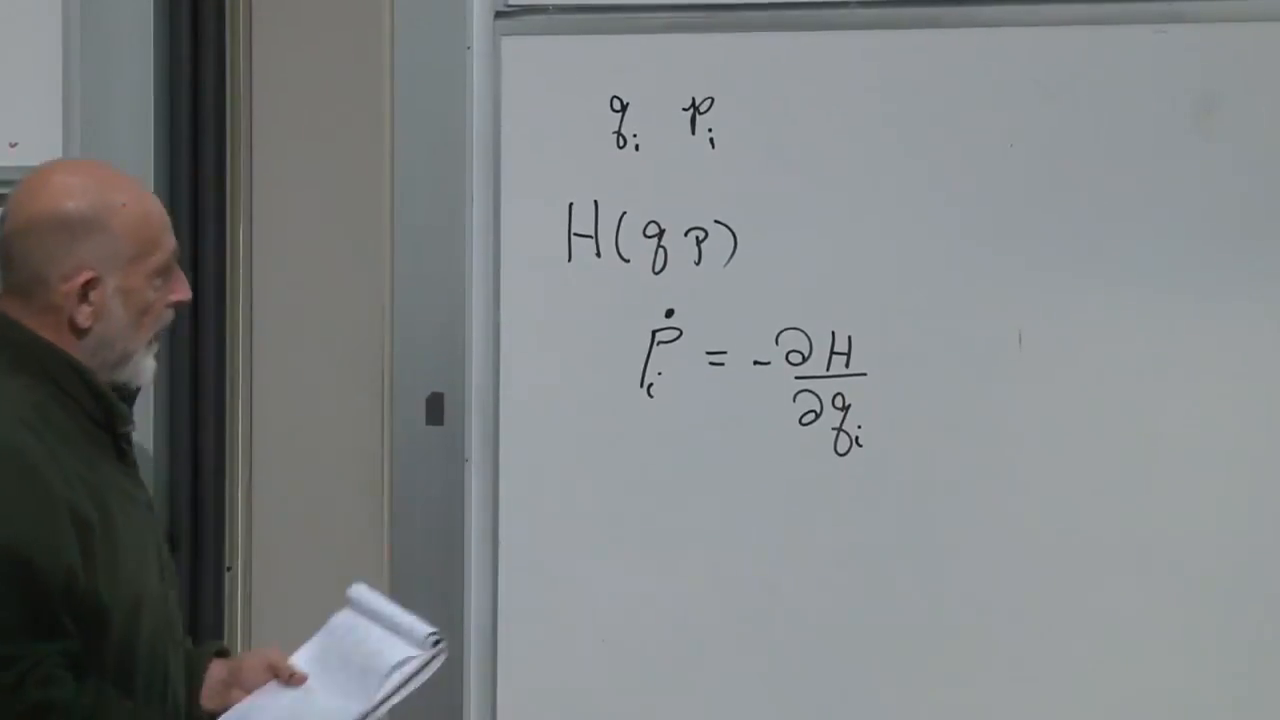
\includegraphics[width=0.82\textwidth]{lecture_07_figure_02.png}
  \caption{Kanonische Variablen, die Funktion \(H(q,p)\) und die Impulsgleichung Hamiltons zu Beginn der Wiederholung.}
  \lectureframe{00:07:29}
\end{figure}

Obwohl die Gleichungen paarweise indiziert sind, muss sich die Dynamik nicht für jedes Paar getrennt beschreiben lassen. Der Hamiltonian kann alle \(q_i\) und \(p_i\) miteinander koppeln, sodass etwa \(\dot p_1\) vom Zustand des gesamten Systems abhängen kann.

\begin{classroomqa}
  \audiencequestion{Ist die Darstellung nun axiomatisch? Welche Beziehung zwischen
  \(p\) und \(q\) wurde vorausgesetzt?
  \lecturetimestamp{00:17:08--00:18:18}}
  \lecturerresponse{Die Hamilton-Gleichungen legen die formale Theorie fest, sobald
  \(H(q,p)\) und die kanonischen Paare spezifiziert sind. Es gibt keine allgemeingültige
  zusätzliche Annahme \(p=m\dot q\). Diese Beziehung gilt für ein gewöhnliches
  kartesisches Teilchen mit quadratischer kinetischer Energie, doch andere Koordinaten und
  andere Hamilton-Funktionen führen zu anderen Impuls--Geschwindigkeits-Beziehungen. Die Gleichungen
  selbst liefern die Beziehung durch
  \(\dot q_i=\partial H/\partial p_i\). Ob ein vorgeschlagener Hamiltonian
  in der Natur realisiert ist, ist eine weitere physikalische Frage.}
\end{classroomqa}

Nun können wir die Energieerhaltung mit einer Argumentation in einer Zeile herleiten. Entlang einer Bahn lautet die totale Ableitung von \(H\)
\begin{equation}
  \frac{dH}{dt}
  =
  \sum_i\left(
    \frac{\partial H}{\partial q_i}\dot q_i
    +\frac{\partial H}{\partial p_i}\dot p_i
  \right)
  +\frac{\partial H}{\partial t}.
  \label{eq:l7-total-h-derivative}
\end{equation}
Der letzte Term beschreibt die explizite Zeitabhängigkeit bei festgehaltenen \(q\) und \(p\), etwa weil sich ein von außen vorgegebener Parameter ändert. Setzen wir Gleichung~\eqref{eq:l7-hamilton-equations} ein, erhalten wir
\begin{align}
  \frac{dH}{dt}
  &=
  \sum_i\left[
    \frac{\partial H}{\partial q_i}
    \frac{\partial H}{\partial p_i}
    -\frac{\partial H}{\partial p_i}
    \frac{\partial H}{\partial q_i}
  \right]
  +\frac{\partial H}{\partial t}\\
  &=\frac{\partial H}{\partial t}.
  \label{eq:l7-h-energy-rate}
\end{align}
Jeder Summand hebt seinen Gegenpart auf. Folglich gilt
\begin{equation}
  \frac{\partial H}{\partial t}=0
  \quad\Longrightarrow\quad
  \frac{dH}{dt}=0.
  \label{eq:l7-energy-conservation}
\end{equation}
Für ein abgeschlossenes, zeittranslationsinvariantes System ist der Hamiltonian erhalten und entspricht der Energie.

\begin{classroomqa}
  \audiencequestion{Was ändert sich, wenn der Hamiltonian explizit von der Zeit abhängt? \lecturetimestamp{00:10:32--00:12:33}}
  \lecturerresponse{Dann gilt Gleichung~\eqref{eq:l7-h-energy-rate} weiterhin, doch die Energie des Teilsystems muss nicht konstant sein. Eine explizite Zeitabhängigkeit steht gewöhnlich für einen nicht berücksichtigten Antrieb, der Energie mit dem System austauscht. Wird dieser Antrieb als dynamischer Teil in ein größeres abgeschlossenes System aufgenommen, kann der Hamiltonian des Gesamtsystems wieder zeitunabhängig und dessen Gesamtenergie erhalten sein.}
\end{classroomqa}

\section{Energie als Geometrie im Phasenraum}

Nehmen wir nun an, \(H\) habe keine explizite Zeitabhängigkeit. Die Anfangsbedingung legt einen Wert \(E\) fest, und der Phasenraumpunkt bleibt auf
\begin{equation}
  H(q,p)=E.
  \label{eq:l7-energy-surface}
\end{equation}
Der Phasenraum hat \(2n\) Dimensionen. An regulären Punkten definiert eine Gleichung unter seinen Koordinaten eine Hyperfläche der Dimension \((2n-1)\). Verschiedene Werte von \(E\) ergeben verschiedene Hyperflächen. Sie müssen weder geschlossen noch kompakt sein; die Energieerhaltung besagt lediglich, dass eine Bahn, die auf einer solchen Fläche beginnt, sie nie verlässt.

Für den angepassten harmonischen Oszillator aus der vorangegangenen Vorlesung gilt
\begin{equation}
  H=\frac{\omega}{2}(p^2+q^2).
  \label{eq:l7-oscillator-hamiltonian}
\end{equation}
Jede Menge konstanter Energie ist also ein Kreis,
\begin{equation}
  p^2+q^2=\frac{2E}{\omega}.
  \label{eq:l7-oscillator-circle}
\end{equation}

\begin{figure}[htbp]
  \centering
  \includegraphics[width=0.84\textwidth]{lecture_07_figure_04.png}
  \caption{Die Phasenraumskizze der Dimension \(2n\) und der Hamiltonian des harmonischen Oszillators, mit denen Flächen konstanter Energie eingeführt werden.}
  \lectureframe{00:15:20}
\end{figure}

Die Bewegungsgleichungen
\begin{equation}
  \dot q=\omega p,\qquad \dot p=-\omega q,
  \label{eq:l7-oscillator-flow}
\end{equation}
lassen den Punkt im Uhrzeigersinn um seinen Kreis laufen. Die Energiegleichung gibt an, auf welcher Kurve die Bewegung verläuft; Hamiltons Gleichungen bestimmen Richtung und Geschwindigkeit entlang dieser Kurve.

\begin{figure}[htbp]
  \centering
  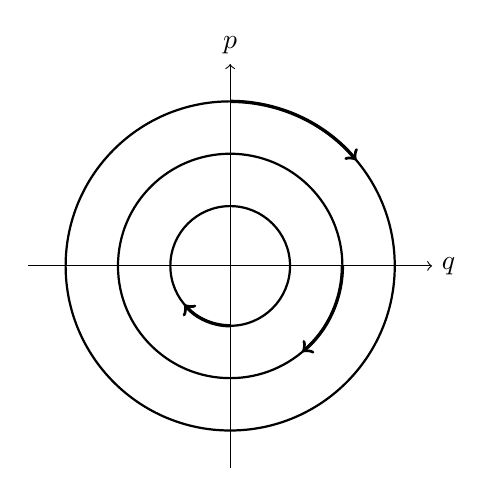
\begin{tikzpicture}[scale=0.95]
    \draw[->] (-2.7,0) -- (2.7,0) node[right] {\(q\)};
    \draw[->] (0,-2.7) -- (0,2.7) node[above] {\(p\)};
    \draw[thick] (0,0) circle (0.8);
    \draw[thick] (0,0) circle (1.5);
    \draw[thick] (0,0) circle (2.2);
    \draw[->,very thick] (0,2.2) arc[start angle=90,end angle=40,radius=2.2];
    \draw[->,very thick] (1.5,0) arc[start angle=0,end angle=-50,radius=1.5];
    \draw[->,very thick] (0,-0.8) arc[start angle=-90,end angle=-140,radius=0.8];
  \end{tikzpicture}
  \caption{Konstante Energie ergibt die Kreise; die Oszillatorgleichungen liefern das tangentiale Strömungsfeld im Uhrzeigersinn.}
\end{figure}

\begin{classroomqa}
  \audiencequestion{Sind Hamiltons beide Gleichungen und \(H=E\) verschiedene Fassungen derselben Gleichung?
  \lecturetimestamp{00:15:53--00:17:06}}
  \lecturerresponse{Nein. Hamiltons Gleichungen sind die beiden Bewegungsgesetze erster Ordnung für ein kanonisches Paar. Sie implizieren \(dH/dt=0\), woraus \(H=E\) folgt. Der Wert von \(E\) wird durch die Anfangsbedingung festgelegt. Die Gleichung \(H=E\) bestimmt eine Fläche; für sich genommen legt sie die Geschwindigkeit entlang dieser Fläche nicht fest.}
\end{classroomqa}

\section{Von einem Zustand zu einem Fluss von Zuständen}

Statt einer einzelnen Anfangsbedingung zu folgen, verteilen wir alle möglichen Anfangsbedingungen über den Phasenraum und lassen die Zeit verstreichen. Jeder Punkt ist ein vollständiger möglicher Zustand, und jeder Zustand entwickelt sich gemäß Hamiltons Gleichungen. Man kann sich diese Verteilung als Staub oder als imaginäres Fluid vorstellen. Dabei wird keine materielle Substanz in den Phasenraum gegossen; das Fluid ist eine Veranschaulichung, mit der sich alle Bahnen zugleich erfassen lassen.

Das Geschwindigkeitsfeld im Phasenraum ist
\begin{equation}
  \mathbf V(q,p,t)
  =
  (\dot q_1,\ldots,\dot q_n,\dot p_1,\ldots,\dot p_n).
  \label{eq:l7-phase-velocity}
\end{equation}
Für ein kanonisches Paar schreiben wir
\begin{equation}
  V_q=\dot q=\frac{\partial H}{\partial p},
  \qquad
  V_p=\dot p=-\frac{\partial H}{\partial q}.
  \label{eq:l7-phase-components}
\end{equation}
An jedem Punkt ordnet der Hamiltonian einen Vektor zu, der dem Phasenraumpunkt seine nächste Bewegungsrichtung vorgibt. Ist \(H\) zeitunabhängig, ist das Vektorfeld stationär: Kehrt man zum selben Phasenraumpunkt zurück, erhält man dieselbe Geschwindigkeit. Hängt \(H\) von der Zeit ab, ändert sich auch das Vektorfeld mit der Zeit, doch es ist zu jedem Zeitpunkt definiert.

\begin{figure}[htbp]
  \centering
  \includegraphics[width=0.84\textwidth]{lecture_07_figure_05.png}
  \caption{Das Geschwindigkeitsfeld des harmonischen Oszillators. Die Vektoren sind tangential zu den Kreisen und werden zum Ursprung hin kürzer.}
  \lectureframe{00:24:50}
\end{figure}

Beim harmonischen Oszillator dreht sich jeder Radius mit der Winkelgeschwindigkeit \(\omega\). Punkte nahe dem Ursprung haben eine geringere lineare Geschwindigkeit, weil sie in derselben Periode einen kürzeren Kreis durchlaufen. Der gesamte Staub rotiert daher wie ein starrer Kreisel.

\begin{classroomqa}
  \audiencequestion{Bedeutet die starre Rotation, dass alle Bahnen des Oszillators dieselbe Periode haben? \lecturetimestamp{00:21:10--00:21:42}}
  \lecturerresponse{Ja. Diese Amplitudenunabhängigkeit ist die definierende besondere Eigenschaft des harmonischen Oszillators. Jeder Kreis wird mit derselben Kreisfrequenz \(\omega\) durchlaufen, obwohl der Betrag der Geschwindigkeit im Phasenraum auf einem kleineren Kreis geringer ist.}
\end{classroomqa}

\begin{classroomqa}
  \audiencequestion{Ist die Geschwindigkeit im Phasenraum an jedem Punkt gleich?
  \lecturetimestamp{00:24:29--00:25:37}}
  \lecturerresponse{Nein. Sowohl ihre Richtung als auch ihr Betrag ändern sich im Allgemeinen mit dem Ort. Beim Oszillator ist der Vektor tangential zum jeweiligen Kreis und hat den Betrag \(\omega\sqrt{p^2+q^2}\). Ein Vektorfeld bedeutet, dass jedem Punkt ein Vektor zugeordnet ist, nicht dass überall derselbe Vektor steht.}
\end{classroomqa}

\begin{classroomqa}
  \audiencequestion{Was genau sind die Teilchen und die Dichte dieses imaginären Fluids? \lecturetimestamp{00:56:03--00:58:40}}
  \lecturerresponse{Jeder Punkt steht für einen vollständigen Zustand des gesamten mechanischen Systems, nicht für ein einzelnes physisches Teilchen. Fünf Teilchen, die sich in einer Raumdimension bewegen, erfordern fünf Orts- und fünf Impulskoordinaten, also einen zehn-dimensionalen Phasenraum; in drei Dimensionen sind es dreißig Dimensionen. Der Staub ist ein Ensemble alternativer Zustände. Wenn das Fluidbild ablenkt, kann man stattdessen einfach ein Gebiet von Anfangsbedingungen nehmen, jeden Punkt darin entwickeln und sein Phasenraumvolumen vorher und nachher vergleichen.}
\end{classroomqa}

\section{Kompression und Divergenz}

Um zu fragen, ob dieses imaginäre Fluid Volumen verliert, betrachten wir zunächst eine Dimension. Punkte auf einer Geraden bewegen sich mit der Geschwindigkeit \(v(x)\). Zwei benachbarte Punkte im Abstand \(\delta x\) haben einen Geschwindigkeitsunterschied
\begin{equation}
  \delta v \simeq \frac{dv}{dx}\,\delta x.
  \label{eq:l7-one-dimensional-strain}
\end{equation}
Ist \(dv/dx>0\), bewegt sich der vordere Punkt schneller und das Intervall wird gedehnt. Ist \(dv/dx<0\), wird es komprimiert. Eine stationäre inkompressible Strömung in einer Dimension erfüllt daher
\begin{equation}
  \frac{dv}{dx}=0.
  \label{eq:l7-one-dimensional-incompressible}
\end{equation}

\begin{figure}[htbp]
  \centering
  \includegraphics[width=0.84\textwidth]{lecture_07_figure_06.png}
  \caption{Die eindimensionale Herleitung von \(dv/dx\) als lokaler Dehnungs- oder Kompressionsrate.}
  \lectureframe{00:30:20}
\end{figure}

Es gibt zwei gleichwertige Sichtweisen. Man kann einem materiellen Intervall folgen und fragen, ob sich seine Länge ändert. Oder man kann ein kleines Intervall festhalten und fragen, ob pro Zeiteinheit genauso viel hineinfließt wie hinaus. Bei der ersten Sichtweise folgt man dem Fluid, bei der zweiten beobachtet man, wie es vorbeiströmt.

In mehr als einer Dimension kann sich ein Gebiet entlang einer Achse dehnen und entlang einer anderen komprimieren, ohne dass sich sein Gesamtvolumen ändert. Für ein Geschwindigkeitsfeld \(\mathbf V=(V_x,V_y,V_z)\) ist die relevante lokale Rate die Divergenz,
\begin{equation}
  \nabla\cdot\mathbf V
  =
  \frac{\partial V_x}{\partial x}
  +\frac{\partial V_y}{\partial y}
  +\frac{\partial V_z}{\partial z}.
  \label{eq:l7-spatial-divergence}
\end{equation}
Eine positive Divergenz bedeutet lokale Expansion, eine negative lokale Kontraktion; Inkompressibilität liegt vor, wenn
\begin{equation}
  \nabla\cdot\mathbf V=0.
  \label{eq:l7-zero-divergence}
\end{equation}
Gleicher Zu- und Abfluss durch eine festgehaltene kleine Box ist dieselbe lokale Aussage wie die Erhaltung des Volumens einer mitbewegten kleinen Box.

\begin{figure}[htbp]
  \centering
  \includegraphics[width=0.86\textwidth]{lecture_07_figure_07.png}
  \caption{Eine zweidimensionale Box, ihre Strömungskomponenten und die Summe der Ableitungen nach den jeweils zugehörigen Koordinaten, die die Divergenz definiert.}
  \lectureframe{00:35:30}
\end{figure}

\begin{classroomqa}
  \audiencequestion{Geht es um ein Fluid im gewöhnlichen Raum oder um eine Strömung im Phasenraum? \lecturetimestamp{00:34:27--00:34:40}}
  \lecturerresponse{Das Divergenzargument ist zunächst ein allgemeines Argument über Fluide. Wir wenden es auf den gerade-dimensionalen Phasenraum an, dessen Koordinatenrichtungen die \(q_i\) und \(p_i\) und dessen Geschwindigkeitskomponenten die \(\dot q_i\) und \(\dot p_i\) sind.}
\end{classroomqa}

Kehren wir nun zu den diskreten Zustandsabbildungen zurück. In einem umkehrbaren Zyklus führt ein Pfeil in jeden Knoten hinein und einer aus ihm heraus; eine ausgewählte Zustandsmenge enthält bei ihrer Entwicklung weiterhin gleich viele Elemente. In einem Senkenpunkt führen viele Pfeile hinein und zu wenige hinaus; mehrere Alternativen werden ununterscheidbar.

\begin{figure}[htbp]
  \centering
  \includegraphics[width=0.80\textwidth]{lecture_07_figure_08.png}
  \caption{Die diskrete Senke, mit der sich die Divergenz wieder an den Test für umkehrbare Gesetze aus der ersten Vorlesung anknüpfen lässt.}
  \lectureframe{00:40:15}
\end{figure}

Die kontinuierliche Frage lässt sich nun präzise stellen: Hat der Hamiltonsche Fluss Divergenz null, sodass ein kleines Gebiet unterscheidbarer Zustände niemals zu einem kleineren Phasenraumvolumen zusammengedrückt wird?

\section{Der Satz von Liouville}

\begin{theorem}[Liouville's theorem]Für ein glattes Hamiltonsches System hat das kanonische Geschwindigkeitsfeld im Phasenraum Divergenz null:
\begin{equation}
  \sum_i\left(
    \frac{\partial\dot q_i}{\partial q_i}
    +\frac{\partial\dot p_i}{\partial p_i}
  \right)=0.
  \label{eq:l7-liouville-divergence}
\end{equation}Äquivalent dazu erhält die Hamiltonsche Entwicklung das kanonische Phasenraumvolumenelement \(dq_1\cdots dq_n\,dp_1\cdots dp_n\).
\end{theorem}

\begin{classroomqa}
  \audiencequestion{Sind die Komponenten namens \(V\) einfach die Zeitableitungen von \(p\) und \(q\)? \lecturetimestamp{00:42:20--00:43:22}}
  \lecturerresponse{Ja. Für ein Paar gilt \(V_q=\dot q\) und \(V_p=\dot p\). Ordnet man alle diese Ableitungen passend an, erhält man den Geschwindigkeitsvektor des Flusses im vollständigen Phasenraum.}
\end{classroomqa}

Für ein kanonisches Paar folgen aus Hamiltons Gleichungen
\begin{equation}
  V_p=-\frac{\partial H}{\partial q},
  \qquad
  V_q=\frac{\partial H}{\partial p}.
  \label{eq:l7-liouville-components}
\end{equation}
Damit lautet die Divergenz
\begin{align}
  \frac{\partial V_p}{\partial p}
  +\frac{\partial V_q}{\partial q}
  &=
  -\frac{\partial}{\partial p}
    \left(\frac{\partial H}{\partial q}\right)
  +\frac{\partial}{\partial q}
    \left(\frac{\partial H}{\partial p}\right)\\
  &=
  -\frac{\partial^2H}{\partial p\,\partial q}
  +\frac{\partial^2H}{\partial q\,\partial p}
  =0.
  \label{eq:l7-liouville-proof}
\end{align}

\begin{figure}[htbp]
  \centering
  \includegraphics[width=0.86\textwidth]{lecture_07_figure_09.png}
  \caption{Das Rechteck mit endlichen Differenzen veranschaulicht, weshalb sich glatte gemischte partielle Ableitungen vertauschen lassen.}
  \lectureframe{00:47:30}
\end{figure}

Die Gleichheit gemischter partieller Ableitungen lässt sich anhand von vier benachbarten Punkten \(A,B,C,D\) an den Ecken eines kleinen Rechtecks in der \(q\)-\(p\)-Ebene veranschaulichen. Bildet man zunächst die Differenz nach \(q\) und anschließend die nach \(p\), ergibt sich bis auf die beiden kleinen Seitenlängen
\begin{equation}
  F(B)+F(D)-F(A)-F(C).
  \label{eq:l7-finite-difference-combination}
\end{equation}
Bildet man die Differenzen in umgekehrter Reihenfolge, erhält man dieselbe Kombination. Im Grenzfall eines kleinen Rechtecks ergibt sich
\(\partial_p\partial_qF=\partial_q\partial_pF\), sofern die erforderlichen Ableitungen stetig sind.

\begin{figure}[htbp]
  \centering
  \includegraphics[width=0.88\textwidth]{lecture_07_figure_10.png}
  \caption{Die kanonische Divergenz, nachdem Hamiltons Gleichungen sie auf zwei gemischte Ableitungen mit entgegengesetzten Vorzeichen zurückgeführt haben.}
  \lectureframe{00:50:20}
\end{figure}

Bei vielen Freiheitsgraden erfolgt dieselbe Aufhebung für jedes kanonische Paar:
\begin{align}
  \sum_i\left(
    \frac{\partial\dot p_i}{\partial p_i}
    +\frac{\partial\dot q_i}{\partial q_i}
  \right)
  &=
  \sum_i\left(
    -\frac{\partial^2H}{\partial p_i\,\partial q_i}
    +\frac{\partial^2H}{\partial q_i\,\partial p_i}
  \right)\\
  &=0.
  \label{eq:l7-many-pair-proof}
\end{align}
Die Dehnung in einer kanonischen Richtung wird durch die Kompression in der zu ihr konjugierten Richtung ausgeglichen. Diese paarweise Aufhebung ist eine stärkere Struktur als eine zufällige Aufhebung zwischen nicht zusammengehörigen Achsen.

\begin{classroomqa}
  \audiencequestion{Wird die Summe über alle kanonischen Paare mitverstanden?
  \lecturetimestamp{00:52:00--00:52:36}}
  \lecturerresponse{Ja. Gleichung~\eqref{eq:l7-many-pair-proof} wird über \(i\) summiert, und die beiden gemischten Ableitungen heben sich für jedes \(q_i,p_i\)-Paar einzeln auf.}
\end{classroomqa}

\begin{classroomqa}
  \audiencequestion{Sieht die dargestellte Divergenz nach einer kartesischen Darstellung aus. Gilt der Satz auch nach einem Koordinatenwechsel?
  \lecturetimestamp{00:52:50--00:53:22,\allowbreak\ 00:58:18--00:58:40}}
  \lecturerresponse{Die natürliche Formulierung verwendet kanonische Koordinaten und das kanonische Volumenelement \(dq_1\cdots dq_n\,dp_1\cdots dp_n\). Eine kanonische, also symplektische Transformation ändert Koordinaten und Impulse gemeinsam und erhält dieses Volumen. Bei beliebigen nichtkanonischen Koordinaten muss ein Jacobi-Faktor in das Volumenmaß eingehen; das naive Produkt der Koordinatendifferentiale muss nicht invariant sein.}
\end{classroomqa}

\begin{classroomqa}
  \audiencequestion{Erfordert der Satz von Liouville einen zeitunabhängigen Hamiltonian? \lecturetimestamp{00:53:43--00:55:51}}
  \lecturerresponse{Nein. Für die Energieerhaltung war \(\partial H/\partial t=0\) erforderlich, doch im Beweis der Divergenz wird nur nach \(q_i\) und \(p_i\) bei festgehaltener Zeit abgeleitet. Für \(H(q,p,t)\) heben sich die gemischten Ableitungen weiterhin auf. Ein zeitabhängiger Hamiltonian erzeugt daher einen zeitabhängigen, aber zu jedem Zeitpunkt volumenbewahrenden kanonischen Fluss.}
\end{classroomqa}

\section{Was Volumenerhaltung bedeutet und was nicht}

Nehmen wir ein beliebiges kleines Gebiet \(R_0\) von Anfangsbedingungen und entwickeln jeden Punkt darin um eine Zeit \(t\) weiter. Der Satz von Liouville besagt
\begin{equation}
  \operatorname{Vol}(R_t)=\operatorname{Vol}(R_0).
  \label{eq:l7-volume-preservation}
\end{equation}
Das Gebiet kann sich verschieben, drehen, scheren und zu einem langen Filament dehnen. Geschützt ist sein Volumen, nicht seine Form. Bei einer glatten Hamiltonschen Entwicklung in endlicher Zeit können verschiedene Phasenraumpunkte nicht zusammenfallen.

Für endliche Zeiten ist ein glatter Hamiltonscher Fluss eine invertierbare Abbildung mit einer glatten Umkehrabbildung, die durch Rückwärtsentwicklung entsteht. Damit lässt sich auch die im Unterricht aufgestellte Behauptung erklären, dass ein zusammenhängender Klumpen nicht in getrennte Stücke zerreißen kann: Der Fluss verformt das Gebiet kontinuierlich und erhält seine Topologie, auch wenn ein extrem dünner Hals bei endlicher Auflösung zwei Lappen getrennt erscheinen lassen kann.

\begin{figure}[htbp]
  \centering
  \includegraphics[width=0.86\textwidth]{lecture_07_figure_12.png}
  \caption{Mögliche Verformungen eines Phasenraumgebiets. Ein glatter Hamiltonscher Fluss kann einen dünnen Hals erzeugen, aber das Gebiet in endlicher Zeit nicht tatsächlich in unabhängig entwickelte Stücke zerreißen.}
  \lectureframe{01:04:55}
\end{figure}

\begin{classroomqa}
  \audiencequestion{Kann ein Phasenraumgebiet abschnüren und in zwei Stücke zerfallen? \lecturetimestamp{01:04:10--01:05:49}}
  \lecturerresponse{Nicht unter einem glatten deterministischen Hamiltonschen Fluss in endlicher Zeit. An einem hypothetischen Abschnürungspunkt gibt es weiterhin einen Phasenraumpunkt mit einer zugeordneten Geschwindigkeit, nicht zwei unvereinbare Richtungen. Das Gebiet kann ein sehr langes, schmales Verbindungsfilament entwickeln, doch die Entwicklung bleibt eineindeutig und zerreißt es nicht.}
\end{classroomqa}

\begin{classroomqa}
  \audiencequestion{Sind zwei weit voneinander entfernte Lappen eines gedehnten Klumpens physisch verbunden oder quantenverschränkt?
  \lecturetimestamp{01:08:01--01:09:16}}
  \lecturerresponse{Eine solche physische Verbindung ist damit nicht gemeint. Der Klumpen ist eine Menge alternativer Anfangsbedingungen, kein einzelnes materielles Objekt. Ihn als ein Gebiet zu bezeichnen, hält fest, dass die Zustände aus derselben gemeinsamen Menge hervorgegangen sind; über Kräfte oder Quantenverschränkung zwischen ihnen sagt das nichts aus.}
\end{classroomqa}

\begin{classroomqa}
  \audiencequestion{Was geschieht nahe dem aufrechten instabilen Gleichgewicht eines starren Pendels? Überlagern sich Bewegungen im Uhrzeigersinn und gegen den Uhrzeigersinn?
  \lecturetimestamp{01:07:07--01:07:47}}
  \lecturerresponse{Benachbarte Anfangsbedingungen können sich auf sehr unterschiedliche Bahnen auseinanderentwickeln und so die beschriebenen dünnen Filamente bilden. Sie werden nicht zu demselben Phasenraumpunkt: Das Vorzeichen der infinitesimalen Auslenkung oder des Impulses unterscheidet die beiden Seiten. Für den exakt ausgeglichenen Zustand ist die Bewegung eindeutig bestimmt; im idealen Modell bleibt er im Gleichgewicht.}
\end{classroomqa}

\subsection{Expansion im Ortsraum und Kontraktion im Impulsraum}

Wenn eine kanonische Transformation einen Ortsbereich um den Faktor \(a\) ausdehnt, verkleinert sich die Skala des konjugierten Impulses um den reziproken Faktor:
\begin{equation}
  q\longrightarrow aq,
  \qquad
  p\longrightarrow \frac{p}{a},
  \qquad
  dq\,dp\longrightarrow dq\,dp.
  \label{eq:l7-canonical-scaling}
\end{equation}
Das ist der klare Phasenrauminhalt des Beispiels mit der Gasexpansion. Bei einer adiabatischen Expansion wächst der zugängliche Bereich im gewöhnlichen Raum, während typische Impulse abnehmen und das Gas abkühlt. Eine genaue thermodynamische Beziehung hängt von der Dimension, dem Expansionsprotokoll und den Wechselwirkungen ab; der Satz von Liouville liefert die Volumenbedingung, nicht jeden thermodynamischen Koeffizienten.

\begin{classroomqa}
  \audiencequestion{Gilt dieselbe Argumentation auch für ein expandierendes Universum, selbst bei einer plötzlichen Expansion? \lecturetimestamp{00:53:23--00:56:00}}
  \lecturerresponse{Der Satz von Liouville gilt immer dann, wenn die vollständige Dynamik Hamiltonsch ist, auch bei explizit zeitabhängigen kanonischen Variablen. Eine Expansion in Ortsrichtungen muss von der entsprechenden Kontraktion in kanonischen Impulsrichtungen begleitet sein. Die kosmologische Skalenexpansion, die kontrollierte Expansion eines Gases und eine frei explodierende Wolke sind jedoch nicht derselbe physikalische Prozess. Eine Hubble-ähnliche Korrelation zwischen Abstand und Fluchtgeschwindigkeit kann entstehen, weil sich schnellere Objekte weiter bewegen, während adiabatische Abkühlung die Kontraktion der lokalen Impulsverteilung betrifft. Der Satz schränkt in beiden Fällen die vollständige Abbildung im Phasenraum ein.}
\end{classroomqa}

\begin{classroomqa}
  \audiencequestion{Welchen praktischen Nutzen hat der Satz von Liouville?
  \lecturetimestamp{01:06:16--01:07:04}}
  \lecturerresponse{Er ist für die statistische Mechanik zentral. Er bestimmt, wie sich Ensembles mikroskopischer Zustände entwickeln, und liegt der Beziehung zwischen Phasenraumvolumen und Entropie zugrunde. Die Expansion und Abkühlung eines Gases ist ein unmittelbares Beispiel; später wird der Satz zu einem grundlegenden Werkzeug für Überlegungen zum Gleichgewicht und Nichtgleichgewicht.}
\end{classroomqa}

\section{Ein Fluss, der die Form stark verändert}

Der harmonische Oszillator erhält sowohl Fläche als auch Form, weil sein Fluss eine starre Drehung ist. Das ist ein Sonderfall. Um Volumenerhaltung von Starrheit zu unterscheiden, betrachten wir
\begin{equation}
  H=\lambda pq,
  \label{eq:l7-pq-hamiltonian}
\end{equation}
wobei \(\lambda\) die Einheit einer inversen Zeit hat. In der Vorlesung wird \(\lambda=1\) gesetzt; wenn wir es beibehalten, bleiben die Dimensionen ausdrücklich sichtbar.

\begin{figure}[htbp]
  \centering
  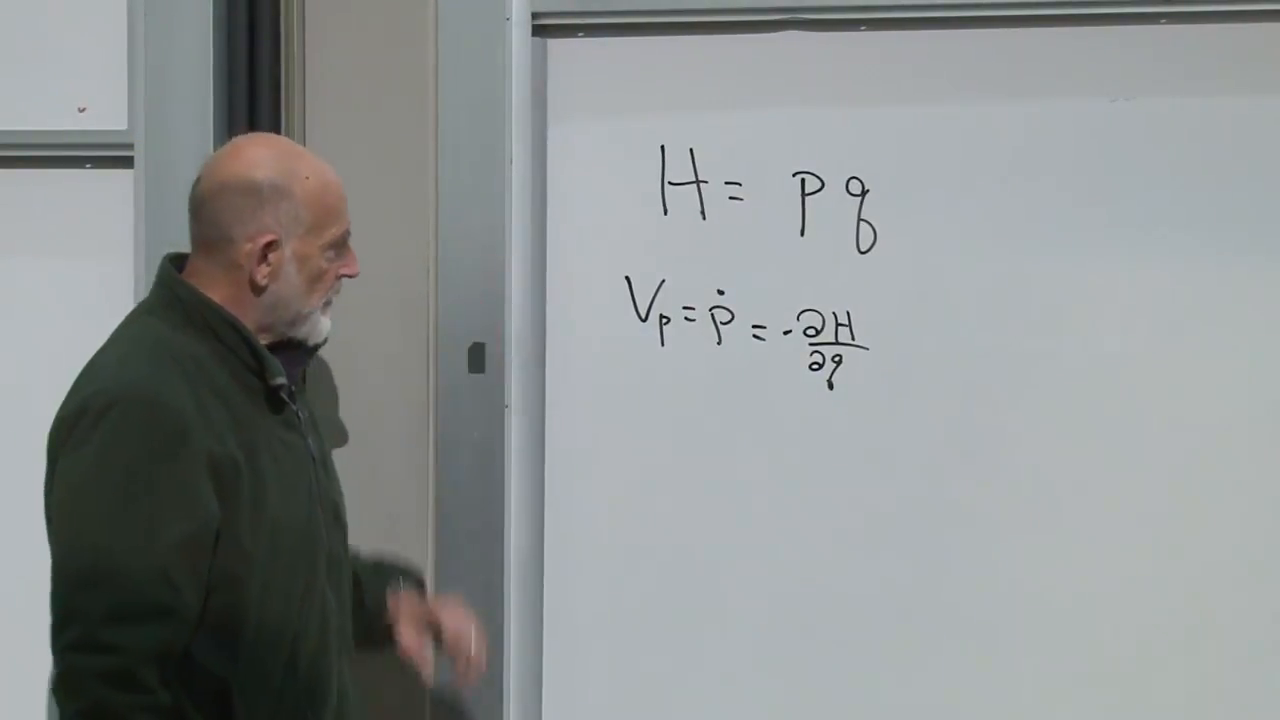
\includegraphics[width=0.82\textwidth]{lecture_07_figure_03.png}
  \caption{Beginn des Beispiels mit \(H=pq\) und erste Komponente der Geschwindigkeit im Phasenraum.}
  \lectureframe{01:00:11}
\end{figure}

Hamiltons Gleichungen lauten
\begin{equation}
  \dot p=-\lambda p,
  \qquad
  \dot q=\lambda q,
  \label{eq:l7-pq-flow}
\end{equation}
mit den Lösungen
\begin{equation}
  p(t)=p_0e^{-\lambda t},
  \qquad
  q(t)=q_0e^{\lambda t}.
  \label{eq:l7-pq-solutions}
\end{equation}
Ein quadratisches Gebiet wird in \(p\) exponentiell gestaucht und um denselben Faktor in \(q\) gedehnt:
\begin{equation}
  \Delta p(t)\Delta q(t)
  =
  \Delta p(0)\Delta q(0).
  \label{eq:l7-pq-area}
\end{equation}
Die Divergenz bestätigt das Ergebnis lokal,
\begin{equation}
  \frac{\partial\dot p}{\partial p}
  +\frac{\partial\dot q}{\partial q}
  =-\lambda+\lambda=0.
  \label{eq:l7-pq-divergence}
\end{equation}

\begin{figure}[htbp]
  \centering
  \includegraphics[width=0.86\textwidth]{lecture_07_figure_11.png}
  \caption{Ein kompaktes Gebiet wird zu einem langen, dünnen Streifen gedehnt, während der Fluss mit \(H=pq\) die Fläche erhält.}
  \lectureframe{01:02:10}
\end{figure}

\begin{classroomqa}
  \audiencequestion{Da \(pq\) die Einheit einer Wirkung hat, bedeutet der Satz von Liouville dann die Erhaltung der Wirkung? \lecturetimestamp{01:03:00--01:04:09}}
  \lecturerresponse{Nein. Der Satz besagt die Erhaltung des Phasenraumvolumens. Bei einem kanonischen Paar hat \(dq\,dp\) die Einheit einer Wirkung; diese Dimensionsbeziehung deutet die Quantenmechanik an, in der Phasenraumzellen in Einheiten gemessen werden, die durch \(\hbar\) festgelegt sind. Das Produkt \(pq\) ist jedoch weder selbst Hamiltons Wirkungsfunktional noch automatisch ein Drehimpuls, nur weil die Einheiten übereinstimmen.}
\end{classroomqa}

Das Beispiel zeigt außerdem, dass Winkel nicht erhalten bleiben müssen. Ein rechtwinkliges Kreuz mit ungleichen Komponenten wird durch die Skalierung in Gleichung~\eqref{eq:l7-pq-solutions} in seiner metrischen Gestalt geschert, während die Fläche erhalten bleibt. Der Satz von Liouville ist ein Flächen- oder Volumensatz, kein Satz über gewöhnliche euklidische Starrheit.

\section{Dämpfung erzeugt eine Senke}

Um zu sehen, was der Satz ausschließt, betrachten wir die reduzierte Gleichung für einen gedämpften Oszillator,
\begin{equation}
  m\ddot x=-kx-c\dot x,
  \qquad c>0.
  \label{eq:l7-damped-newton}
\end{equation}
Sei \(p=m\dot x\). Dann gilt
\begin{equation}
  \dot x=\frac{p}{m},
  \qquad
  \dot p=-kx-\frac{c}{m}p.
  \label{eq:l7-damped-first-order}
\end{equation}
Ohne Dämpfung umläuft der Phasenraumpunkt den Ursprung. Mit Dämpfung wird Energie auf die mikroskopischen Freiheitsgrade des umgebenden Mediums übertragen, und die Bahn windet sich spiralförmig nach innen.

\begin{figure}[htbp]
  \centering
  \includegraphics[width=0.84\textwidth]{lecture_07_figure_13.png}
  \caption{Die Gleichung des gedämpften Oszillators und seine nach innen verlaufende Spirale in der \(x\)-\(p\)-Ebene.}
  \lectureframe{01:13:30}
\end{figure}

Die Divergenz dieses reduzierten zweidimensionalen Flusses ist
\begin{equation}
  \frac{\partial\dot x}{\partial x}
  +\frac{\partial\dot p}{\partial p}
  =
  0-\frac{c}{m}<0.
  \label{eq:l7-damped-divergence}
\end{equation}
Jedes Gebiet endlicher Ausdehnung schrumpft. Der Ursprung ist ein Senkenpunkt, das kontinuierliche Gegenstück zur Zustandsabbildung, in die viele Pfeile hineinführen.

\begin{figure}[htbp]
  \centering
  \includegraphics[width=0.88\textwidth]{lecture_07_figure_14.png}
  \caption{Die Geschwindigkeitskomponenten des gedämpften Flusses im Phasenraum, aus denen die negative Divergenz \(-c/m\) folgt.}
  \lectureframe{01:16:05}
\end{figure}

Das bedeutet nicht, dass die mikroskopische Mechanik den Satz von Liouville verletzt. Die beiden Variablen \(x,p\) lassen die ungeheuer vielen Freiheitsgrade der Umgebung außer Acht, die die Energie des Oszillators aufnehmen. Das erweiterte System aus Oszillator und Umgebung kann Hamiltonsch sein und das Volumen erhalten, obwohl seine reduzierte Beschreibung in den Variablen \(x,p\) kontrahiert.

\begin{classroomqa}
  \audiencequestion{Wird der gedämpfte Oszillator weiterhin durch die Newton-Gleichung beschrieben, obwohl er in diesem reduzierten Phasenraum nicht Hamiltonsch ist?
  \lecturetimestamp{01:20:09--01:21:12}}
  \lecturerresponse{Ja. Die Newton-Gleichung \(F=ma\) kann eine empirisch vorgegebene Widerstandskraft enthalten. Die elementare \(L=T-V\)- und Hamilton-Beschreibung gilt unmittelbar für konservative Kräfte; allgemeinere Lagrangefunktionen erfassen auch einige geschwindigkeitsabhängige Kräfte. Ein Markovscher Reibungsterm für ein isoliertes Paar \(x,p\) beschreibt jedoch reduzierte dissipative Dynamik und kein abgeschlossenes kanonisches Hamilton-System.}
\end{classroomqa}

\begin{classroomqa}
  \audiencequestion{Geht wirklich Information verloren, wenn sich die gedämpften Gleichungen mit unendlicher Genauigkeit rückwärts integrieren lassen?
  \lecturetimestamp{01:25:16--01:27:17}}
  \lecturerresponse{Für jede endliche Zeit hat die ideale Differentialgleichung weiterhin eine Umkehrung; exakte Daten lassen sich also rückwärts entwickeln. Die präzise Aussage lautet, dass endliche Phasenraumzellen exponentiell schrumpfen. Um ihren früheren Zustand wiederherzustellen, ist daher exponentiell zunehmende Genauigkeit erforderlich; im Grenzfall unendlicher Zeit nähern sich alle Trajektorien dem Senkenpunkt. Dies ist die nächstliegende kontinuierliche klassische Analogie zum diskreten Bild des Verlusts von Alternativen, aber keine Behauptung, zwei exakte Lösungen würden sich zu endlicher Zeit buchstäblich vereinigen.}
\end{classroomqa}

\begin{classroomqa}
  \audiencequestion{Kann ein Vektorfeld eine verschwindende Divergenz haben, ohne aus einem Hamilton-System hervorzugehen? \lecturetimestamp{01:18:21--01:22:34}}
  \lecturerresponse{Gewiss. Die Hamilton-Form ist hinreichend für eine verschwindende Divergenz, aber nicht notwendig. Ein beliebiges inkompressibles Geschwindigkeitsfeld kann eine verschwindende Divergenz haben, ohne auf demselben Raum ein kanonisches Hamiltonsches Vektorfeld zu sein. Das dreidimensionale Geschwindigkeitsfeld einer inkompressiblen Flüssigkeit ist das Lehrbuchbeispiel: Drei Koordinaten können für sich genommen keine kanonischen Paare bilden. Die vollständige Fluidmechanik kann zwar anspruchsvollere Hamilton-Formulierungen mit unendlich vielen Freiheitsgraden besitzen, doch ändert das nichts an der hier behaupteten einseitigen Implikation.}
\end{classroomqa}

\section{Weitere durch Fragen verdeutlichte Unterscheidungen}

\begin{classroomqa}
  \audiencequestion{Wie hängt die Bewegung auf einer Fläche konstanter Energie mit der Erhaltung eines ganzen Phasenraumvolumens zusammen?
  \lecturetimestamp{01:28:47--01:30:41}}
  \lecturerresponse{Beides sind unabhängige Folgen der Hamilton-Struktur. Ist \(H\) zeitunabhängig, bleibt jede Trajektorie auf ihrer eigenen Energiefläche. Ein endlicher Bereich kann viele solcher Flächen durchqueren; der Satz von Liouville besagt, dass das Volumen dieses gesamten Bereichs erhalten bleibt. Beim harmonischen Oszillator bleibt auch die Form des Bereichs erhalten, weil die Strömung eine starre Rotation ist. Der Bereich für \(H=pq\) behält dagegen nur seine Fläche, nicht seine Form.}
\end{classroomqa}

\begin{classroomqa}
  \audiencequestion{Welche Rolle spielt die mechanische Arbeit in der Hamilton-Beschreibung? \lecturetimestamp{01:30:44--01:32:57}}
  \lecturerresponse{Arbeit beschreibt Energie, die über eine gewählte Systemgrenze übertragen wird. Ein äußerer Akteur kann ein Gewicht anheben oder einen Parameter ändern und dadurch die Energie des Teilsystems verändern; die von ihm zugeführte Energie verliert der Akteur. Werden beide Seiten in ein einziges abgeschlossenes Modell aufgenommen, stehen wieder die Erhaltung der Gesamtenergie und der Austausch zwischen Teilsystemen im Vordergrund.}
\end{classroomqa}

\begin{classroomqa}
  \audiencequestion{Erhält die Volumenerhaltung auch die Topologie und die Winkel?
  \lecturetimestamp{01:33:00--01:33:37}}
  \lecturerresponse{Eine glatte Hamiltonsche Strömung zu endlicher Zeit erhält die Topologie, da sie eine umkehrbare stetige Verformung ist. Euklidische Winkel oder die Form bleiben im Allgemeinen nicht erhalten. Bei der Rotation des Oszillators ist das zwar der Fall, doch die Streckung für \(H=pq\) zeigt, warum dies ein Sonderfall ist.}
\end{classroomqa}

\begin{classroomqa}
  \audiencequestion{Wurde die Legendre-Transformation ausgelassen, weil sie keine physikalische Bedeutung hat? \lecturetimestamp{01:33:43--01:34:48}}
  \lecturerresponse{Nein. Sie ist die nützliche Transformation, die die Geschwindigkeitsbeschreibung in eine Impulsbeschreibung überführt und bei regulärer Abbildung \(H=\sum_i p_i\dot q_i-L\) ergibt. Die Konstruktion wurde bereits wiederholt verwendet, auch wenn ihr formaler Name nicht hervorgehoben wurde; die ausführliche allgemeine Theorie wird für den vorliegenden Satz einfach nicht benötigt.}
\end{classroomqa}

\section{Poisson-Klammern: die nächste Verdichtung}

In den letzten Minuten kehren wir zum historischen Thema zurück. Die Mechanik des 19. Jahrhunderts suchte wiederholt nach kompakten Strukturen, die scheinbar unterschiedliche Systeme miteinander verbanden---Mechanik und geometrische Optik, Teilchen und Strahlen, klassische Trajektorien und wellenartige Beschreibungen. Poisson-Klammern sind eine weitere solche Struktur und werden in der Quantenmechanik besonders wichtig.

Sei \(F(q,p)\) eine beliebige Funktion auf dem Phasenraum. Sie kann eine Koordinate, ein Impuls, das Produkt \(qp\) oder der Drehimpuls sein. Entlang der Bewegung gilt
\begin{equation}
  \frac{dF}{dt}
  =
  \sum_i\left(
    \frac{\partial F}{\partial q_i}\dot q_i
    +\frac{\partial F}{\partial p_i}\dot p_i
  \right).
  \label{eq:l7-f-time-derivative}
\end{equation}
Setzt man die Hamilton-Gleichungen ein, erhält man
\begin{equation}
  \frac{dF}{dt}
  =
  \sum_i\left(
    \frac{\partial F}{\partial q_i}
    \frac{\partial H}{\partial p_i}
    -
    \frac{\partial F}{\partial p_i}
    \frac{\partial H}{\partial q_i}
  \right).
  \label{eq:l7-f-hamiltonian-derivative}
\end{equation}

\begin{figure}[htbp]
  \centering
  \includegraphics[width=0.88\textwidth]{lecture_07_figure_15.png}
  \caption{Die Kettenregel für die Zeitableitung einer allgemeinen Phasenraumfunktion \(F(q,p)\).}
  \lectureframe{01:42:40}
\end{figure}

Die wiederholt auftretende antisymmetrische Kombination verdient einen eigenen Namen. Für zwei beliebige Funktionen \(F\) und \(G\) definieren wir ihre Poisson-Klammer durch
\begin{equation}
  \boxed{
  \{F,G\}
  =
  \sum_i\left(
    \frac{\partial F}{\partial q_i}
    \frac{\partial G}{\partial p_i}
    -
    \frac{\partial F}{\partial p_i}
    \frac{\partial G}{\partial q_i}
  \right).}
  \label{eq:l7-poisson-bracket}
\end{equation}

\begin{figure}[htbp]
  \centering
  \includegraphics[width=0.86\textwidth]{lecture_07_figure_16.png}
  \caption{Die Ableitungskombination zweier Funktionen, aufgefasst als Poisson-Klammer.}
  \lectureframe{01:44:15}
\end{figure}

Gleichung~\eqref{eq:l7-f-hamiltonian-derivative} wird zu
\begin{equation}
  \boxed{\frac{dF}{dt}=\{F,H\}.}
  \label{eq:l7-hamiltonian-poisson-evolution}
\end{equation}
Hängt \(F\) zusätzlich explizit von der Zeit ab, kommt \(\partial F/\partial t\) hinzu. Für \(F=q_i\) oder \(F=p_i\) erhält man wieder die beiden Hamilton-Gleichungen; Gl.~\eqref{eq:l7-hamiltonian-poisson-evolution} ist somit eine kompakte Form der vollständigen Dynamik.

Die Notation lässt sich immer künstlich verdichten---man könnte viele Gleichungen quadrieren, addieren und das Ergebnis eine einzige Gleichung nennen. Damit würde man die Struktur verbergen, statt sie sichtbar zu machen. Die Poisson-Klammer ist aus dem entgegengesetzten Grund nützlich: Ihre Algebra ordnet die zeitliche Entwicklung, Erhaltungsgrößen und Symmetrien. Als Nächstes entwickeln wir diese Algebra und wenden sie dann auf den Drehimpuls an, dessen Struktur sowohl in der klassischen Mechanik als auch in der Quantentheorie zentral sein wird.

\section{Die kontinuierliche Bedeutung der Umkehrbarkeit}

Wir können die Gedankenkette nun vollständig formulieren. Die Hamilton-Gleichungen erhalten \(H\), wenn der Hamiltonian nicht explizit von der Zeit abhängt; einzelne Trajektorien bleiben daher auf Energiehyperflächen konstanten Energiewerts. Dieselben Gleichungen ordnen jedem Punkt des Phasenraums eine Geschwindigkeit zu. Die Divergenz dieses Geschwindigkeitsfelds verschwindet, weil sich gemischte partielle Ableitungen paarweise aufheben. Folglich bleibt das kanonische Volumen eines ganzen Zustandsraums erhalten.

Das ist die kontinuierliche Version von einem Pfeil hinein und einem Pfeil hinaus. Die Form kann sich ändern, Winkel können sich ändern, und benachbarte Trajektorien können sich enorm voneinander entfernen. Was in einer glatten, abgeschlossenen Hamilton-Beschreibung nicht geschehen kann, ist die Kompression einer endlichen Menge von Alternativen auf ein kleineres Phasenraumvolumen. Die Strömung für \(H=pq\) zeigt, dass Streckung möglich ist; der reduzierte gedämpfte Oszillator veranschaulicht die Senke, die auftritt, sobald die Hamilton-Bedingungen aufgegeben werden. Die Poisson-Klammern verdichten dieselbe Dynamik schließlich zu der Aussage, dass der Hamiltonian jede Zeitableitung erzeugt.
